\vspace{3cm}
\subsubsection{Pagina de autentificare}

\vspace{1cm}
\begin{center}
	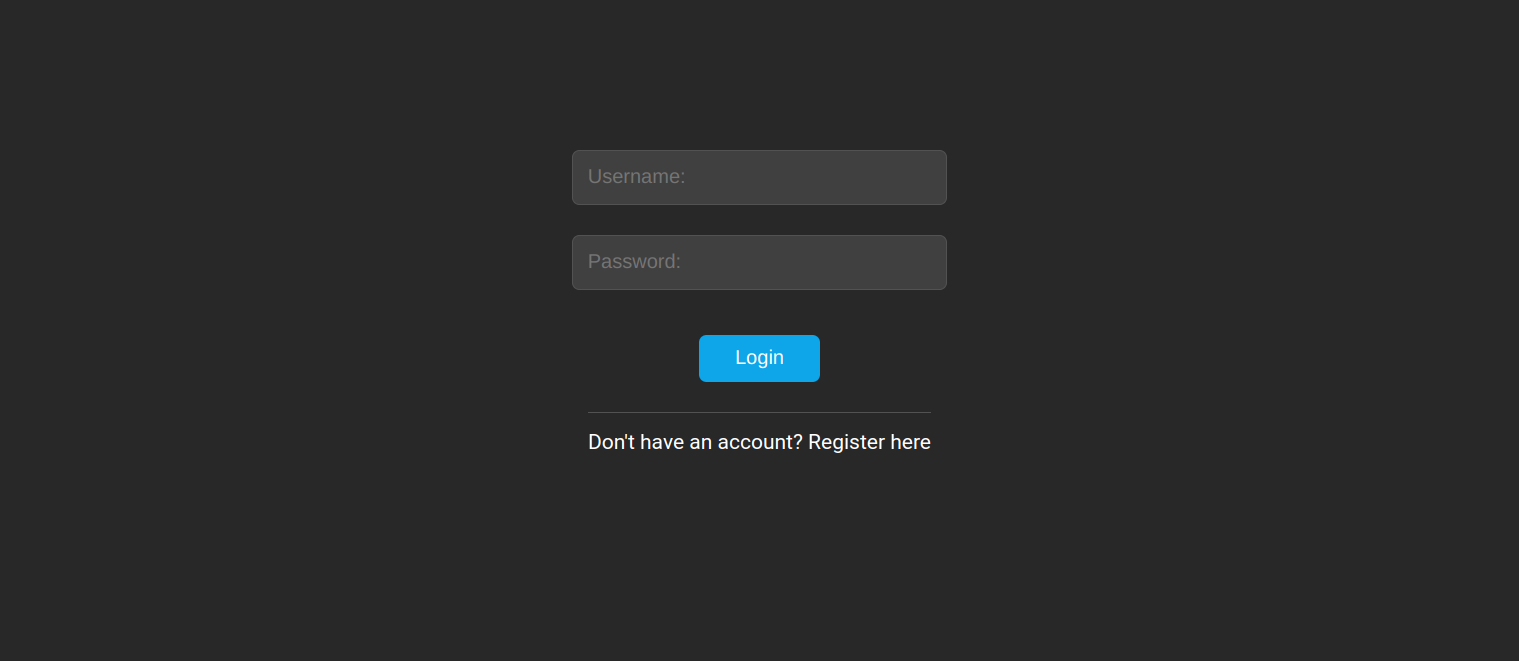
\includegraphics[width=15cm]{3/frontend/login.png}
\end{center}
\vspace{1cm}

\begin{lstlisting}[language=RustHtml]
fn login_form(
    username_value: Option<&str>,
    username_error: Option<&str>,
    password_error: Option<&str>,
) -> String {
    html! {
    <form action="/login" class="register-form" method="post">
        <div class="field-div">
            <input
                type="text"
                id="username"
                name="username"
                placeholder="Username: "
                class="field"
                value={username_value.unwrap_or("")}
                required
            />
            <span class="error">{username_error.unwrap_or("")}</span>
        </div>
        <div class="field-div">
            <input
                type="password"
                id="password"
                name="password"
                placeholder="Password: "
                class="field"
                required
            />
            <span class="error">{password_error.unwrap_or("")}</span>
        </div>
        <button type="submit" class="register-btn">"Login"</button>
    </form>

    <div class="below-form">
        <a href="/register" class="login">"Don't have an account? Register here"</a>
    </div>
    }
}
\end{lstlisting}
